% SafeDischarge — AI6101 mini-project report.
% Build:  ~/.local/bin/tectonic main.tex   (XeLaTeX engine; uses the Arial font installed on macOS)
% Format required by the brief: <= 10 A4 pages, Arial 10pt, reasonable margins,
% including all figures, tables and references.
% Every number in this report comes from prototype/results/*.json (rerun prototype/run_all.sh after code changes).

\documentclass[10pt,a4paper]{article}

% ---------- Page and font ----------
\usepackage[a4paper,margin=2.54cm,footskip=1.0cm]{geometry}
\usepackage{fontspec}
\setmainfont{Arial}[Ligatures=TeX]
\setsansfont{Arial}[Ligatures=TeX]
\setmonofont{Arial}
\setlength{\parindent}{1.2em}
\setlength{\parskip}{1pt}
\widowpenalty=10000
\clubpenalty=10000
\setlength{\emergencystretch}{1.5em}

% ---------- Packages ----------
\usepackage{microtype}
\usepackage{xcolor}
\usepackage{graphicx}
\graphicspath{{../../design/}{../../prototype/results/figures/}}
\usepackage{booktabs,tabularx,array}
\renewcommand{\arraystretch}{1.15}
\usepackage[font=normalsize,labelfont=bf,labelsep=colon,skip=4pt]{caption}
\usepackage{needspace}
\newcommand{\lead}[1]{\needspace{4\baselineskip}\textbf{#1}}
\usepackage{enumitem}
\setlist{nosep,leftmargin=1.5em,topsep=1pt}
\usepackage{titlesec}
\titleformat{\section}{\fontsize{12}{14}\selectfont\bfseries}{\thesection}{0.8em}{}
\titleformat{\subsection}{\fontsize{10}{12}\selectfont\bfseries}{\thesubsection}{0.8em}{}
\titlespacing*{\section}{0pt}{10pt}{4pt}
\titlespacing*{\subsection}{0pt}{7pt}{3pt}
\usepackage[hidelinks]{hyperref}
\usepackage{xurl}
\hypersetup{pdftitle={SafeDischarge: Fair, Explainable and Privacy-Preserving Readmission Risk Prediction},
            pdfauthor={Nguyen Hoang Truong Giang}}

% Let floats fill pages more fully
\renewcommand{\topfraction}{0.9}
\renewcommand{\bottomfraction}{0.8}
\renewcommand{\textfraction}{0.1}
\renewcommand{\floatpagefraction}{0.8}
\setlength{\textfloatsep}{8pt plus 2pt minus 2pt}
\setlength{\floatsep}{8pt plus 2pt minus 2pt}

% Abstract at full 10pt size (LaTeX's default abstract is 9pt), indented like a paper
\renewenvironment{abstract}{\begin{list}{}{\leftmargin=2em\rightmargin=2em\topsep=0pt}\item\relax\textbf{Abstract.}\ }{\end{list}}

\begin{document}

% ---------- Title block (team name, members, emails) ----------
\begin{center}
{\fontsize{15}{18.5}\selectfont\bfseries\hyphenpenalty=10000\exhyphenpenalty=10000
SafeDischarge: Fair, Explainable and Privacy-Preserving\\Readmission Risk Prediction for Diabetic Patients\par}
\vspace{8pt}
\textbf{Team:} SafeDischarge\\[2pt]
Nguyen Hoang Truong Giang \textperiodcentered{} HOANGTRU003@e.ntu.edu.sg\\[2pt]
Code: \url{https://github.com/jilkabe/safedischarge}
\end{center}

\vspace{2pt}
\begin{abstract}
Diabetic inpatients are often readmitted within 30 days of discharge, but follow-up resources such as nurse calls and early appointments are limited. We present \textbf{SafeDischarge}, a discharge-planning assistant that ranks patients by 30-day readmission risk at a fixed follow-up capacity, explains each flag with reasons linked to follow-up actions, and is trained across hospitals without pooling patient records. On the public Diabetes 130-US Hospitals dataset (99,340 stays), a tuned gradient-boosting model places 40.8\% of readmissions in the top 20\% of the list, double the yield of random selection. All three Responsible AI practices are implemented and measured. \emph{Explainability:} SHAP reasons pass a faithfulness test; removing a patient's top-3 reasons lowers risk by 29\%, versus 2.7\% for three random variables. \emph{Fairness:} a permutation-tested audit found that patients aged 80+ were under-detected; per-age-group thresholds closed the gap (21.5 → 6.8 points, p\,=\,0.39) at a cost of 1.1 points of recall. \emph{Privacy:} federated learning with secure aggregation nearly matches pooled training (AUROC 0.675 vs 0.677), and differential privacy at ε\,=\,8 reduces a membership-inference attack to chance.

\vspace{3pt}\noindent\textbf{Keywords:} readmission prediction; explainable AI; algorithmic fairness; federated learning; differential privacy
\end{abstract}

\section{Introduction}\label{sec:1}

\subsection{The problem}\label{sec:1.1}

Patients with diabetes are readmitted to hospital more often than other inpatients. Unplanned readmission within 30 days of discharge is costly, often preventable, and a sign that discharge planning or follow-up care was not enough. Hospitals widely use it as a quality indicator. In the United States, the Hospital Readmissions Reduction Program (HRRP) financially penalises hospitals with excess readmissions~\cite{cms-hrrp}.

Interventions that reduce readmission exist and are well understood: medication reconciliation, diabetes education before discharge, an early follow-up appointment, and a nurse phone call within 72 hours. These interventions take staff time, so they cannot be given to everyone. The practical question for a discharge team is therefore:
\begin{quote}\emph{Of the diabetic patients being discharged today, which ones should receive the limited follow-up resources?}\end{quote}

\subsection{Why existing approaches fall short}\label{sec:1.2}
\begin{enumerate}
\item \textbf{Simple scores are coarse.} Hospitals often use rule-based indices such as LACE~\cite{vanwalraven2010} or the HOSPITAL score~\cite{donze2013}. They are transparent but use few variables and have modest accuracy~\cite{kansagara2011}. They ignore diabetes-specific signals such as HbA1c testing or medication changes during the stay.
\item \textbf{Machine-learning models raise trust problems.} More accurate models can be black boxes that nurses will not act on, and they can quietly perform worse for some patient groups~\cite{obermeyer2019,rajkomar2018}.
\item \textbf{Single-hospital data is small.} One hospital has too few readmissions to train a good model, especially for small subgroups. Pooling patient records across hospitals raises privacy, legal and governance barriers.
\end{enumerate}

\subsection{Our solution}\label{sec:1.3}

\textbf{SafeDischarge} is a discharge-planning assistant. Each day it ranks diabetic patients due for discharge by their risk of readmission within 30 days, explains the main factors behind each patient's risk, and suggests a follow-up action for each factor. The discharge nurse uses the list to allocate a fixed number of follow-up slots.

The design is \textbf{practical and implemented}. We built a working prototype on the public \textbf{Diabetes 130-US Hospitals (1999–2008)} dataset~\cite{strack2014} using open-source tools (scikit-learn~\cite{pedregosa2011}, SHAP~\cite{lundberg2017}, Fairlearn~\cite{bird2020}, PyTorch with Opacus~\cite{yousefpour2021}). It includes a nurse dashboard. Every result in this report was measured on that prototype.

\textbf{What is new.} Most readmission models are judged by AUROC alone. SafeDischarge differs in four ways:
\begin{itemize}
\item \textbf{Evaluated where it is used.} Accuracy and fairness are measured at a fixed number of follow-up slots (recall at capacity). This exposed two problems a standard evaluation hides: tie-breaking that changed fairness results (Section~\ref{sec:3.2}), and a fairness-constrained model that became \emph{less} fair at capacity (Section~\ref{sec:4.2}).
\item \textbf{Explanations lead to actions, and are tested.} Each reason maps to a follow-up action, and a faithfulness test shows the reasons are what actually drives each flag (Section~\ref{sec:4.1}).
\item \textbf{A statistical fairness gate.} Permutation tests separate real gaps from noise, so small groups are not passed or failed by chance.
\item \textbf{The three practices tested together.} One release gate re-tests every practice after every change, which revealed interactions: differential privacy narrowed the age gap, and re-weighting by age widened the sex gap.
\end{itemize}

\lead{All three Responsible AI practices are addressed and measured:}
\begin{itemize}
\item \textbf{Explainability:} top-3 reasons per flagged patient, each linked to an action and tested for faithfulness.
\item \textbf{Fairness:} the audit found that patients aged 80+ were under-detected; per-age-group thresholds removed the gap for 1.1 points of recall.
\item \textbf{Privacy:} federated training with secure aggregation and differential privacy nearly matches pooled-data accuracy, with no measurable leakage.
\end{itemize}

\section{Application Description}\label{sec:2}

\subsection{Stakeholders and users}\label{sec:2.1}
\begin{table}[htbp]
\centering
\caption{Stakeholders and their needs.}\label{tab:1}
\begin{tabularx}{\textwidth}{>{\raggedright\arraybackslash\hsize=1.192\hsize}X>{\raggedright\arraybackslash\hsize=0.831\hsize}X>{\raggedright\arraybackslash\hsize=0.977\hsize}X}
\toprule
\textbf{Stakeholder} & \textbf{Role} & \textbf{Key need} \\
\midrule
Discharge nurses and case managers & Main users; allocate follow-up slots & A short ranked list with reasons they can act on \\
Ward physicians & Review flagged patients; adjust discharge plan & Clinically sensible explanations \\
Patients & Receive follow-up support & Fair access to support; protection of their data \\
Hospitals (data custodians) & Run local nodes; join the federation & Data stays on premises; compliance with health-privacy law \\
Model governance committee (clinicians, data-protection officer, equity lead) & Approves each model release & Evidence of accuracy, fairness and privacy \\
\bottomrule
\end{tabularx}
\end{table}


\subsection{System architecture}\label{sec:2.2}

SafeDischarge has three layers (Figure~\ref{fig:1}):
\begin{itemize}
\item \textbf{Hospital node} (inside each hospital's network): feature pipeline, local trainer, scoring service, explanation engine, nurse dashboard.
\item \textbf{Federation server} (run by a neutral party such as a regional health authority): coordinates training rounds, performs secure aggregation, tracks the privacy budget, stores model versions. It never receives patient records or any single hospital's update.
\item \textbf{Governance layer}: fairness and accuracy audit, model cards, release gate and monitoring.
\end{itemize}
\begin{figure}[htbp]
\centering
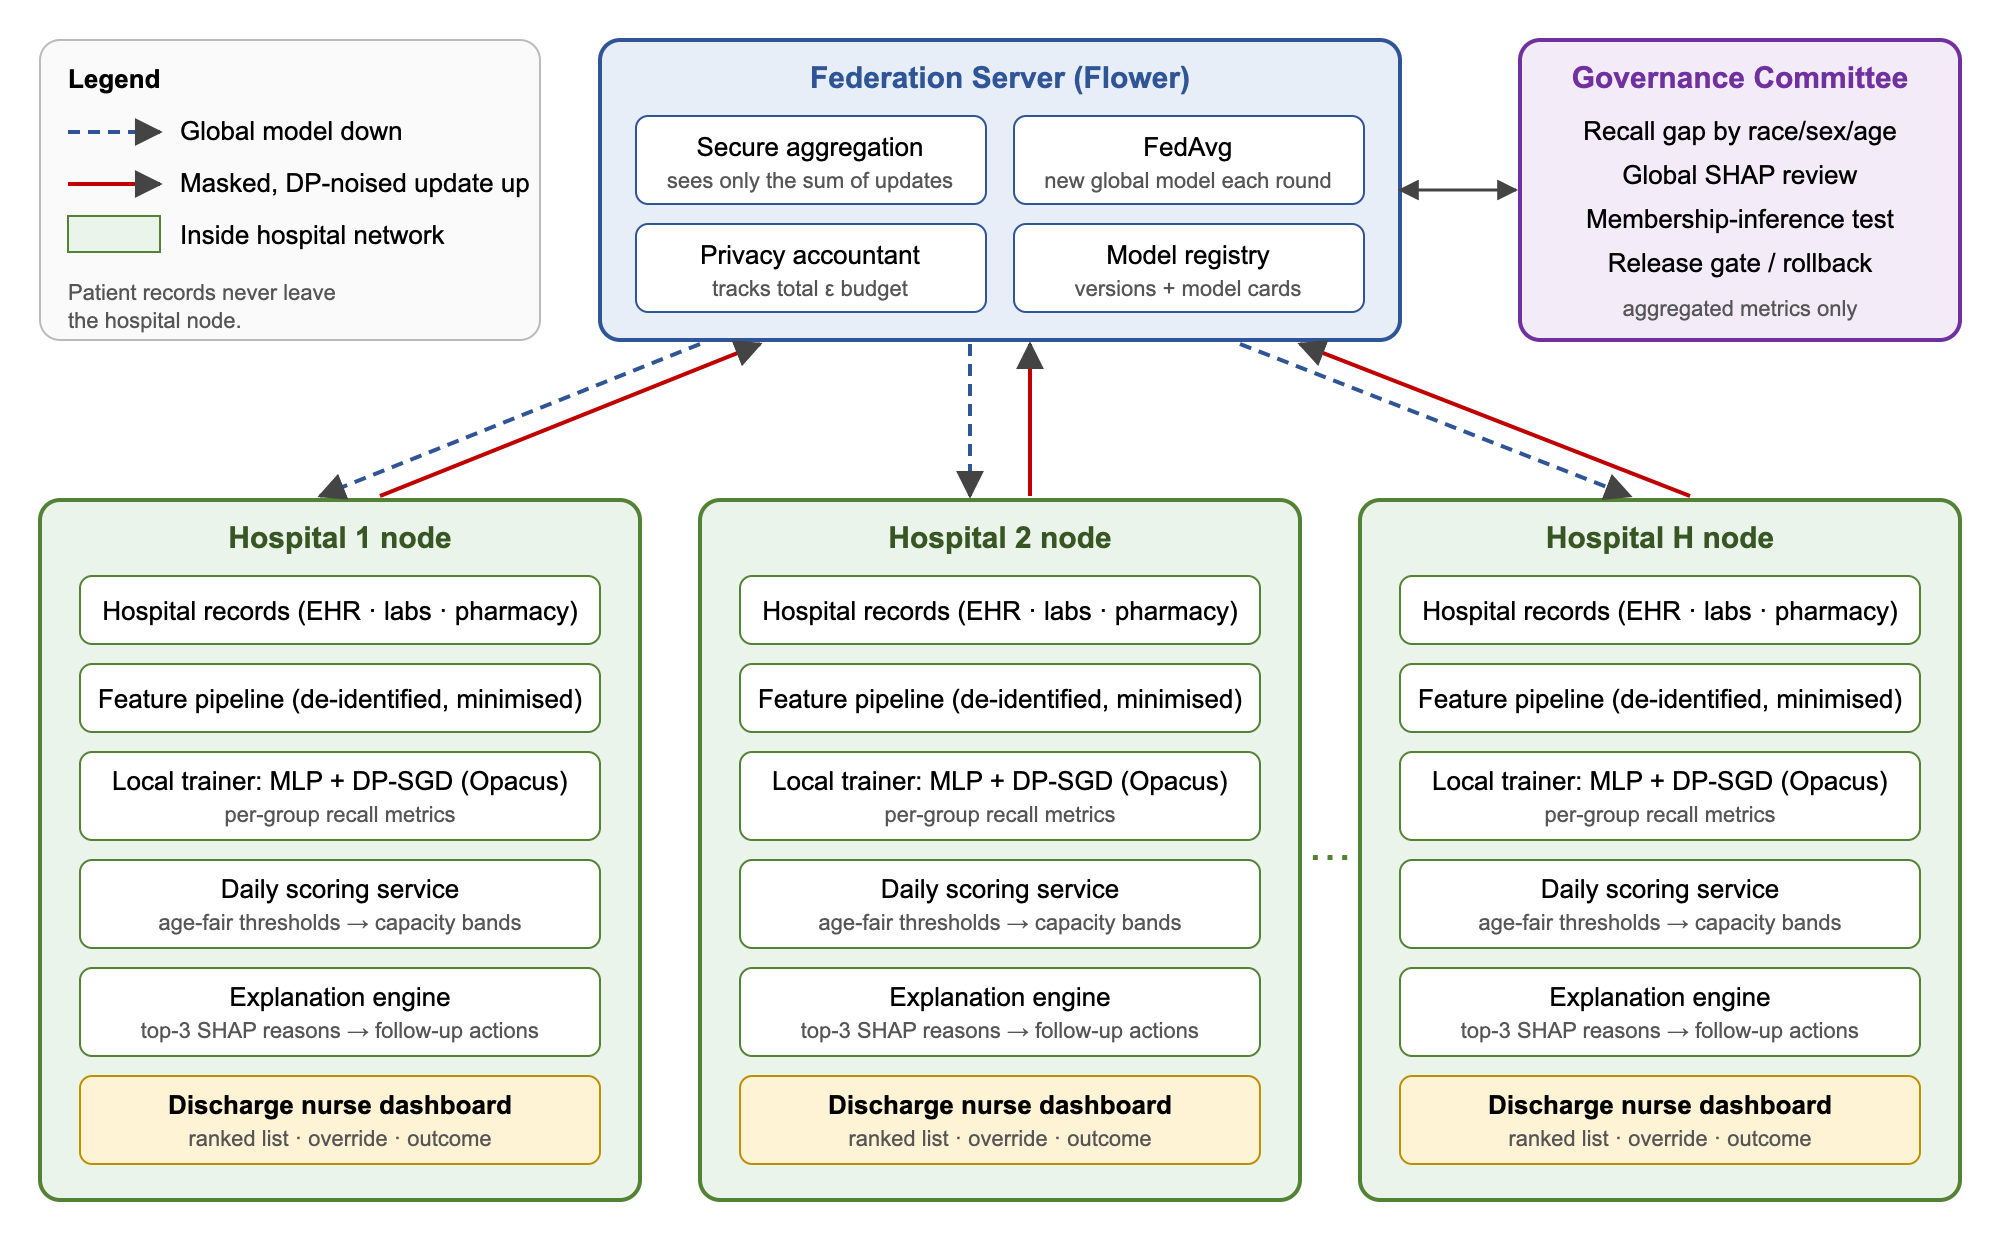
\includegraphics[width=\textwidth]{architecture.png}
\caption{SafeDischarge system architecture.}\label{fig:1}
\end{figure}


\subsection{User journey}\label{sec:2.3}
\begin{enumerate}
\item \textbf{Daily trigger.} Each morning, SafeDischarge scores every diabetic inpatient due for discharge, using data already in the hospital record.
\item \textbf{Ranked list at capacity.} The nurse sets today's number of follow-up slots (\emph{k}). The top-\emph{k} patients are marked “High: follow-up”, the next \emph{k} “Medium”, the rest “Low”. Each patient shows a calibrated 30-day risk (e.g. “25\%”).
\item \textbf{Reasons and actions.} Each flagged patient shows up to three risk factors in plain language, each with a suggested action (Figure~\ref{fig:2}). A real example from the prototype:
\begin{itemize}
\item “3 inpatient admissions in the past year” → \emph{refer to case management}
\item “2 earlier 30-day readmissions” → \emph{review why earlier discharges failed}
\item “Discharge destination: care facility” → \emph{hand-over call to receiving facility}
\end{itemize}
\item \textbf{Decision.} The nurse accepts or overrides each plan. Overrides are logged with a reason.
\item \textbf{Outcome capture.} 30-day readmissions are recorded automatically and become new training data.
\end{enumerate}
\begin{figure}[htbp]
\centering
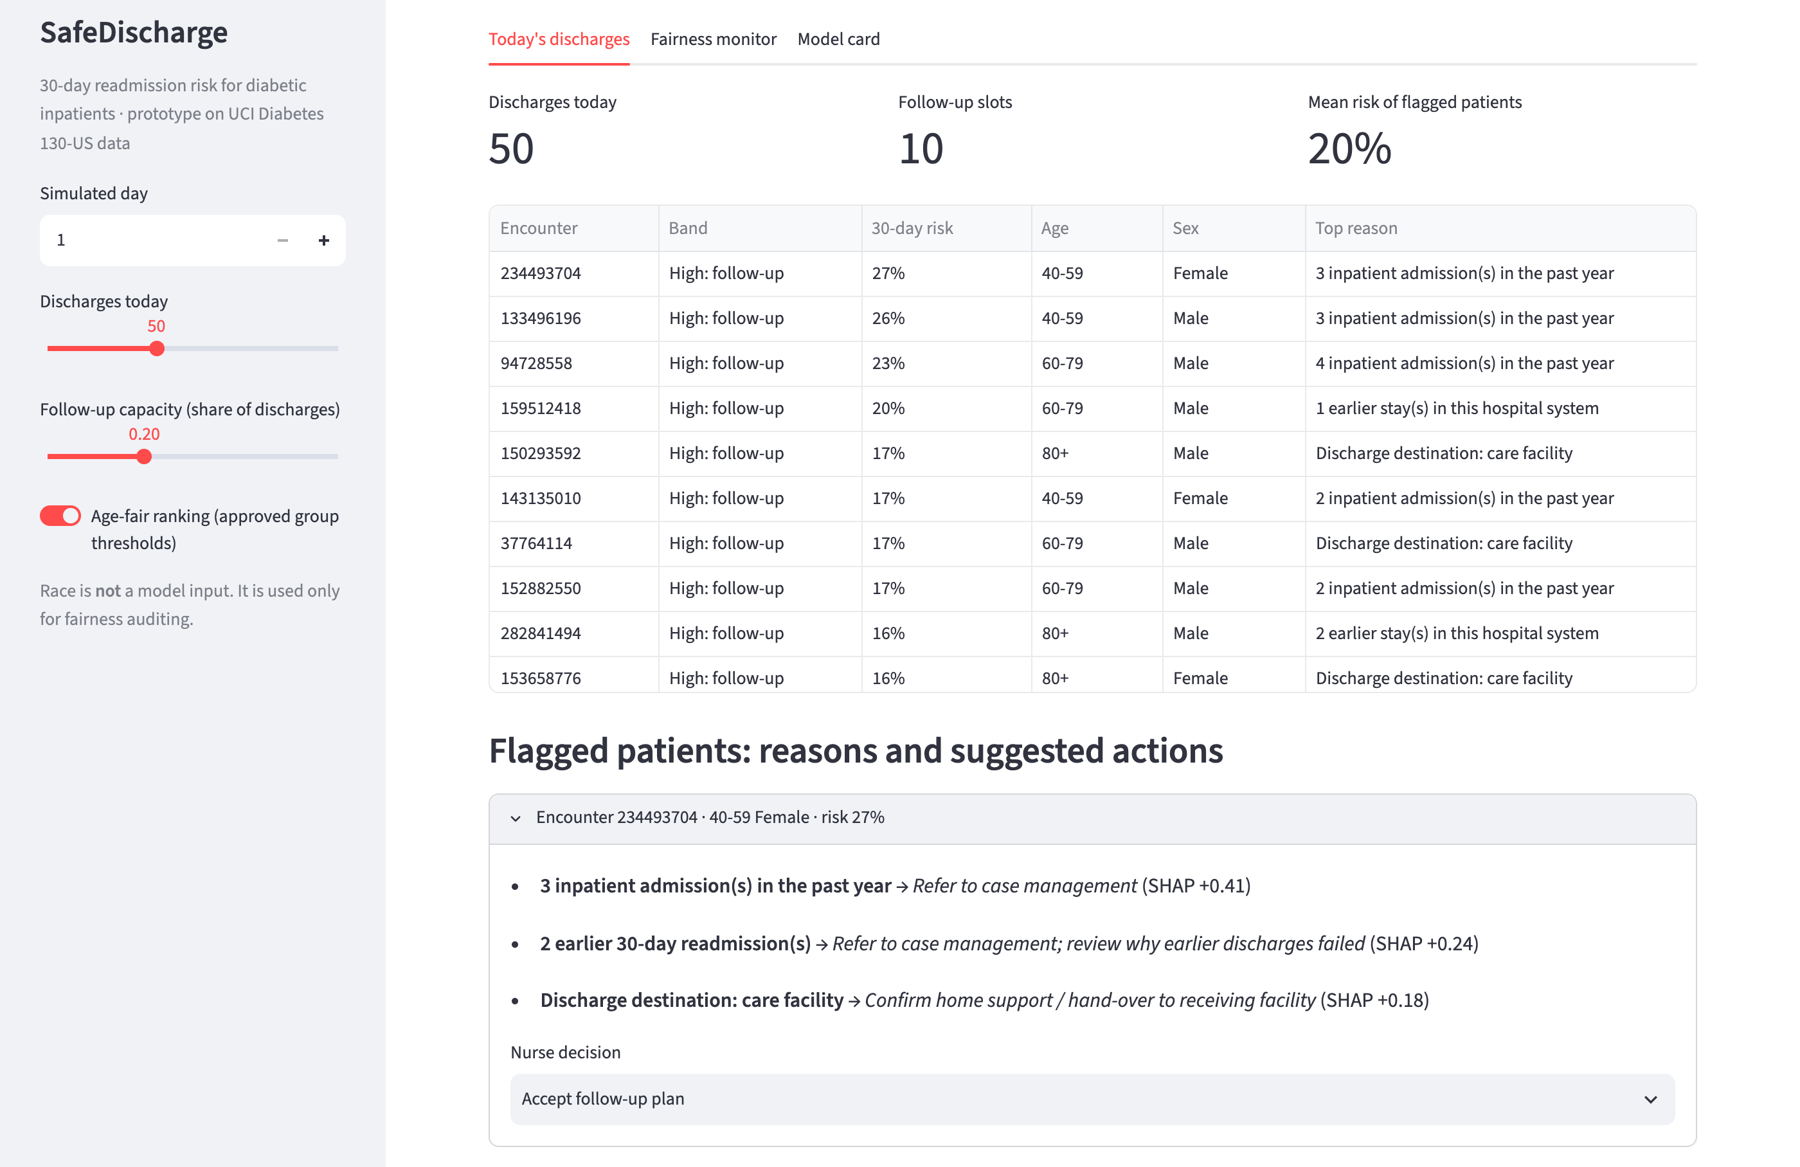
\includegraphics[width=0.78\textwidth]{dashboard.png}
\caption{Prototype nurse dashboard: today's ranked list with calibrated risk and top reason (top), and one flagged patient's three reasons, suggested actions and the nurse's decision (bottom).}\label{fig:2}
\end{figure}


\subsection{Data}\label{sec:2.4}

The \textbf{Diabetes 130-US Hospitals} dataset~\cite{strack2014} (CC BY 4.0) contains 101,766 inpatient stays of 1–14 days with a diabetes diagnosis, from 130 US hospitals. It stands in for the records a real hospital would hold.
\begin{table}[htbp]
\centering
\caption{Data used by SafeDischarge.}\label{tab:2}
\begin{tabularx}{\textwidth}{>{\raggedright\arraybackslash\hsize=0.461\hsize}X>{\raggedright\arraybackslash\hsize=1.580\hsize}X>{\raggedright\arraybackslash\hsize=0.959\hsize}X}
\toprule
\textbf{Group} & \textbf{Fields} & \textbf{Use} \\
\midrule
Demographics & race, sex, age (10-year bands) & Fairness audit groups; age is also a model input. Race is \textbf{not} an input \\
Admission & admission type and source, discharge destination, length of stay & Inputs \\
Prior use & outpatient, emergency and inpatient visits in the past year; the patient's earlier stays in the data and how many of them ended in a 30-day readmission & Inputs \\
Clinical & diagnoses (ICD-9, grouped into 9 clinical categories), number of diagnoses, lab tests, procedures, medications & Inputs \\
Diabetes-specific & HbA1c and glucose test results, insulin and metformin status, number of diabetes medication changes & Inputs; linked to follow-up actions \\
Outcome & readmitted within 30 days & Target (11.4\% positive after exclusions) \\
\bottomrule
\end{tabularx}
\end{table}


\lead{Data preparation decisions:}
\begin{itemize}
\item \textbf{Deaths and hospice.} 2,423 stays ending in death or hospice are excluded, plus 3 with unknown sex. This leaves 99,340 stays from 69,987 patients.
\item \textbf{Earlier stays.} 23\% of patients have more than one stay, so 30\% of stays have an earlier one. For each stay we count the patient's \emph{earlier} stays and earlier 30-day readmissions. The data has no dates, so stay-ID order is used as time order. Only earlier stays are used, and their outcomes are always known by the current discharge, so no future information leaks in. Patients with two earlier readmissions are readmitted 31\% of the time, versus 10\% for those with none.
\item \textbf{Repeat patients.} Splits are made \textbf{by patient} (70/15/15 train/validation/test), so no patient appears in two sets. Splitting by stay would let the model memorise patients and inflate test results.
\item \textbf{Missing data.} \texttt{weight} (97\% missing) is dropped. \texttt{payer\_code} (40\% missing) is kept only as an audit attribute. \texttt{medical\_specialty} (49\% missing) gets an explicit “Unknown” category. HbA1c was not measured in 83\% of stays, and that absence is itself informative, so it is kept as a “not measured” category.
\item \textbf{No hospital ID.} The dataset does not record which hospital each stay came from, so multiple hospitals are \textbf{simulated} (Section~\ref{sec:3.4}).
\end{itemize}

\section{Use of AI Technologies}\label{sec:3}

\subsection{Readmission risk model}\label{sec:3.1}
\begin{itemize}
\item \textbf{Task:} binary classification. Will the patient be readmitted within 30 days, given what is known at discharge?
\item \textbf{Models compared:} L2-regularised logistic regression (the transparent baseline), gradient-boosted trees (scikit-learn HistGradientBoosting~\cite{pedregosa2011}), and a small 2-layer neural network (MLP, used for federated training). All use class weighting because readmissions are the minority class. Gradient-boosting settings were chosen by a 40-trial random search scored on validation AUPRC; the test set was not used for any choice.
\item \textbf{Main metric, recall at capacity:} of all patients actually readmitted, the share who appear in the top 20\% of the ranked list. 20\% is the assumed follow-up capacity. Random selection would give 20\%.
\end{itemize}
\begin{table}[htbp]
\centering
\caption{Model comparison on the held-out test set (14,859 stays, 1,681 readmissions).}\label{tab:3}
\begin{tabularx}{\textwidth}{>{\raggedright\arraybackslash\hsize=1.555\hsize}X>{\raggedright\arraybackslash\hsize=0.637\hsize}X>{\raggedright\arraybackslash\hsize=0.637\hsize}X>{\raggedright\arraybackslash\hsize=1.171\hsize}X}
\toprule
\textbf{Model} & \textbf{AUROC} & \textbf{AUPRC} & \textbf{Recall at 20\% capacity} \\
\midrule
Logistic regression & 0.667 & 0.211 & 36.1\% \\
\textbf{Gradient boosting (chosen)} & \textbf{0.681} & \textbf{0.233} & \textbf{40.8\%} \\
MLP & 0.681 & 0.230 & 39.9\% \\
Gradient boosting + race as input & 0.681 & 0.234 & 40.1\% \\
\bottomrule
\end{tabularx}
\end{table}


\textbf{Reading the results.} Discrimination is modest (AUROC ≈ 0.68), which matches what is generally reported for readmission models~\cite{kansagara2011}. But it doubles the yield of a random selection: about 41\% of future readmissions fall in the top 20\% of the list. Gradient boosting catches 4.6 points more readmissions than logistic regression, about 78 more patients per 1,681. Our rule is to prefer the simpler model unless the complex one adds at least 2 points of recall, so gradient boosting is chosen. Adding race as an input changes nothing (same AUROC, slightly lower recall), so race is left out of the model and used only for auditing.

\subsection{Calibration and capacity-based ranking}\label{sec:3.2}
\begin{itemize}
\item \textbf{Calibration.} Isotonic regression fitted on the validation set turns scores into honest probabilities. The Brier score falls from 0.215 (class-weighted raw scores) to 0.095, slightly better than the 0.100 obtained by predicting the base rate for everyone. The calibrated value is what the nurse sees.
\item \textbf{Ranking on the raw score.} Isotonic calibration maps many patients to the same probability, creating ties. In our first prototype, which patients were flagged at the capacity cut-off, and therefore the fairness results, depended on how those ties were broken. The final design ranks on the model's raw (continuous) score and uses the calibrated probability only for display. This is a practical lesson: fairness checks should be run on exactly the ranking that is deployed.
\end{itemize}

\subsection{Explanation engine}\label{sec:3.3}
\begin{itemize}
\item \textbf{Per-patient explanations:} TreeSHAP~\cite{lundberg2017} values for each prediction. Values for one-hot columns of the same variable are summed, so “discharge destination” counts as one reason. Only factors that \emph{increase} risk are shown.
\item \textbf{Reason → action table:} a short clinician-authored table maps each variable to a follow-up action, e.g. prior inpatient visits → case management; HbA1c not measured → order HbA1c or diabetes clinic review.
\item \textbf{Global check:} SHAP importance ranks prior inpatient admissions first, followed by discharge destination, the patient's earlier stays, age, number of diagnoses and earlier 30-day readmissions. This matches clinical knowledge and published risk indices~\cite{vanwalraven2010,donze2013}, which is evidence that the model relies on sensible signals.
\end{itemize}

\subsection{Federated learning across hospitals}\label{sec:3.4}
\begin{itemize}
\item \textbf{Simulation.} Training patients are assigned to \emph{H} = 5 virtual hospitals. Within each race × age stratum, hospital shares are drawn from a Dirichlet(0.5) distribution, which gives each hospital a very different case mix, as in real networks. Hospital sizes range from 6,518 to 20,524 stays. The African American share ranges from 3\% to 47\%, and the share aged 80+ from 3\% to 35\%.
\item \textbf{Training.} FedAvg~\cite{mcmahan2017}: 20 rounds of 1 local epoch each, with updates weighted by hospital size. In production we would use the Flower framework~\cite{beutel2020}; the prototype implements the same protocol directly in PyTorch for transparency.
\item \textbf{Secure aggregation~\cite{bonawitz2017}.} Each pair of hospitals shares a random mask; one adds it, the other subtracts it. The server sees only masked updates, which are uncorrelated with the real updates (correlation 0.02), but the masks cancel in the sum (maximum error 3 × 10\textsuperscript{−7}). The prototype simulates the key agreement; a real deployment would use the cryptographic protocol of~\cite{bonawitz2017}.
\item \textbf{Results (Table~\ref{tab:4}).} Federated training nearly matches pooling all the data (AUROC 0.675 vs 0.677) and beats every hospital training alone (0.649–0.666, mean 0.660). In other words, hospitals get almost all the benefit of pooled data without pooling it.
\end{itemize}
\begin{table}[htbp]
\centering
\caption{Federated learning and differential privacy (MLP; mean of 3 random seeds; AUROC standard deviation ≤ 0.002, except 0.008 for the over-fitted control).}\label{tab:4}
\begin{tabularx}{\textwidth}{>{\raggedright\arraybackslash\hsize=1.592\hsize}X>{\raggedright\arraybackslash\hsize=0.602\hsize}X>{\raggedright\arraybackslash\hsize=0.712\hsize}X>{\raggedright\arraybackslash\hsize=1.094\hsize}X}
\toprule
\textbf{Setting} & \textbf{AUROC} & \textbf{Recall at 20\%} & \textbf{Membership-inference AUC} \\
\midrule
Each hospital alone (mean of 5) & 0.660 & 37.2\% & – \\
All data pooled (not allowed in practice) & 0.677 & 39.2\% & 0.511 \\
Federated + secure aggregation & 0.675 & 38.8\% & 0.508 \\
+ DP, ε = 8 & 0.662 & 36.9\% & 0.500 \\
+ DP, ε = 3 & 0.657 & 36.2\% & 0.500 \\
+ DP, ε = 1 & 0.644 & 35.1\% & 0.499 \\
Over-fitted control (no DP) & 0.601 & 29.1\% & 0.592 \\
\bottomrule
\end{tabularx}
\end{table}


\subsection{Monitoring and prototype}\label{sec:3.5}

\textbf{Monitoring.} Drift in key features and in the readmission rate is checked monthly. Recall, calibration and the fairness tests are tracked once 30-day outcomes are known (the dashboard's \emph{Fairness monitor} tab). The model is retrained quarterly by federated learning, and each version must pass the release gate (Section~\ref{sec:4.4}).

\textbf{Prototype.} The prototype (\url{https://github.com/jilkabe/safedischarge}) runs every experiment in this report end to end in about 9 minutes on a laptop (\texttt{run\_all.sh}). It covers data preparation and model comparison, the explanation faithfulness test, the fairness audit and mitigations, federated training with DP and the membership-inference attack, and the Streamlit nurse dashboard (Figure~\ref{fig:2}).

\section{Responsible AI Practices Addressed}\label{sec:4}

\subsection{Explainability}\label{sec:4.1}

\textbf{Why it matters:} nurses must decide quickly and will not act on an unexplained score. Explanations also let clinicians catch a model that relies on a wrong or unfair signal.

\lead{Mechanisms (all implemented):}
\begin{enumerate}
\item \textbf{Top-3 reasons per flagged patient} from SHAP, in plain language.
\item \textbf{Reason → action mapping}, so every explanation leads to something the nurse can do.
\item \textbf{Calibrated probabilities}, so “25\% risk” means about 25 in 100 similar patients are readmitted.
\item \textbf{Transparent baseline:} logistic regression is always reported. The complex model is used only if it beats the baseline by a set margin (Section~\ref{sec:3.1}).
\item \textbf{Global review:} SHAP importance is checked against clinical knowledge before each release (Section~\ref{sec:3.3}).
\item \textbf{Model card} in the dashboard: intended use, data, performance, fairness results and limitations.
\end{enumerate}

\textbf{Are the explanations faithful?} An explanation helps only if it reflects what the model actually uses. For each of the 2,972 patients flagged in the test set, we replaced the variables behind their top-3 reasons with values from randomly chosen training patients (averaged over 20 draws) and re-scored them. Their risk score fell by 29\% on average, and 97\% dropped off the flagged list. Replacing 3 randomly chosen variables lowered risk by only 2.7\%, and 15\% dropped off. The top-3 reasons outperformed the random variables for 99\% of patients. The reasons shown to nurses are therefore the factors that actually cause each flag.

\textbf{Further evaluation (not yet done):} a usability test with clinical reviewers. Can they say \emph{why} a patient was flagged, and do they agree with the reason? Target ≥ 80\% agreement.

\subsection{Fairness}\label{sec:4.2}

\textbf{Why it matters:} SafeDischarge decides who gets \emph{extra help}. If high-risk patients in one group are under-detected, that group systematically receives less follow-up care~\cite{obermeyer2019}.

\textbf{Definition.} The harm is \emph{missing} a patient who needed help, so we require \textbf{equal opportunity}~\cite{hardt2016}: recall at capacity should be similar across groups of each protected attribute (race, sex, age). Insurance type is monitored as an audit-only proxy for socio-economic status.

\textbf{Testing for real gaps, not noise.} Some groups are tiny. For example, Asian patients are 0.6\% of stays and have only 7 readmissions in the test set. The largest-minus-smallest recall gap among small groups is dominated by noise, so a fixed tolerance such as “gap ≤ 5 points” would fail or pass largely by chance. For each attribute we therefore run a \textbf{permutation test}: we shuffle group labels among the readmitted patients 2,000 times and ask how often chance alone produces a gap as large as the one observed. Groups with fewer than 30 readmissions are reported with confidence intervals but not tested. They are flagged as needing more data, not declared fair.

\textbf{Audit result.} Race gap: 9.7 points, p = 0.31, not significant. Sex gap: 1.8 points, p = 0.49, not significant. \textbf{Age gap: 21.5 points, p < 0.001, significant.} The model catches 58\% of readmissions in patients under 40 but only \textbf{36\% in patients aged 80+}, the group most vulnerable after discharge. A likely cause is that older patients are readmitted for reasons that are less visible in prior-use counts.

\textbf{Mitigations compared} (Figure~\ref{fig:3}), each also re-tested for race and sex:
\begin{table}[htbp]
\centering
\caption{Fairness mitigation results on the test set (capacity fixed at 20\%).}\label{tab:5}
\begin{tabularx}{\textwidth}{>{\raggedright\arraybackslash\hsize=1.884\hsize}X>{\raggedright\arraybackslash\hsize=0.768\hsize}X>{\raggedright\arraybackslash\hsize=0.805\hsize}X>{\raggedright\arraybackslash\hsize=0.775\hsize}X>{\raggedright\arraybackslash\hsize=0.768\hsize}X}
\toprule
\textbf{Method} & \textbf{Overall recall} & \textbf{Age gap (p)} & \textbf{Sex gap (p)} & \textbf{Release gate} \\
\midrule
Baseline & 40.8\% & 21.5 pts (< 0.001) & 1.8 pts (0.49) & \textbf{Fails} (age) \\
Pre-processing: re-weight under-detected age groups & 39.7\% & 13.5 pts (\textbf{0.02}) & 4.4 pts (0.06) & \textbf{Fails} (age) \\
In-processing: Fairlearn exponentiated gradient, TPR parity~\cite{bird2020} & 32.7\% & 56.6 pts (< 0.001) & 4.1 pts (0.09) & \textbf{Fails} \\
\textbf{Post-processing: per-age-group thresholds} & \textbf{39.7\%} & \textbf{6.8 pts (0.39)} & \textbf{1.7 pts (0.50)} & \textbf{Passes} \\
\bottomrule
\end{tabularx}
\end{table}

\begin{figure}[htbp]
\centering
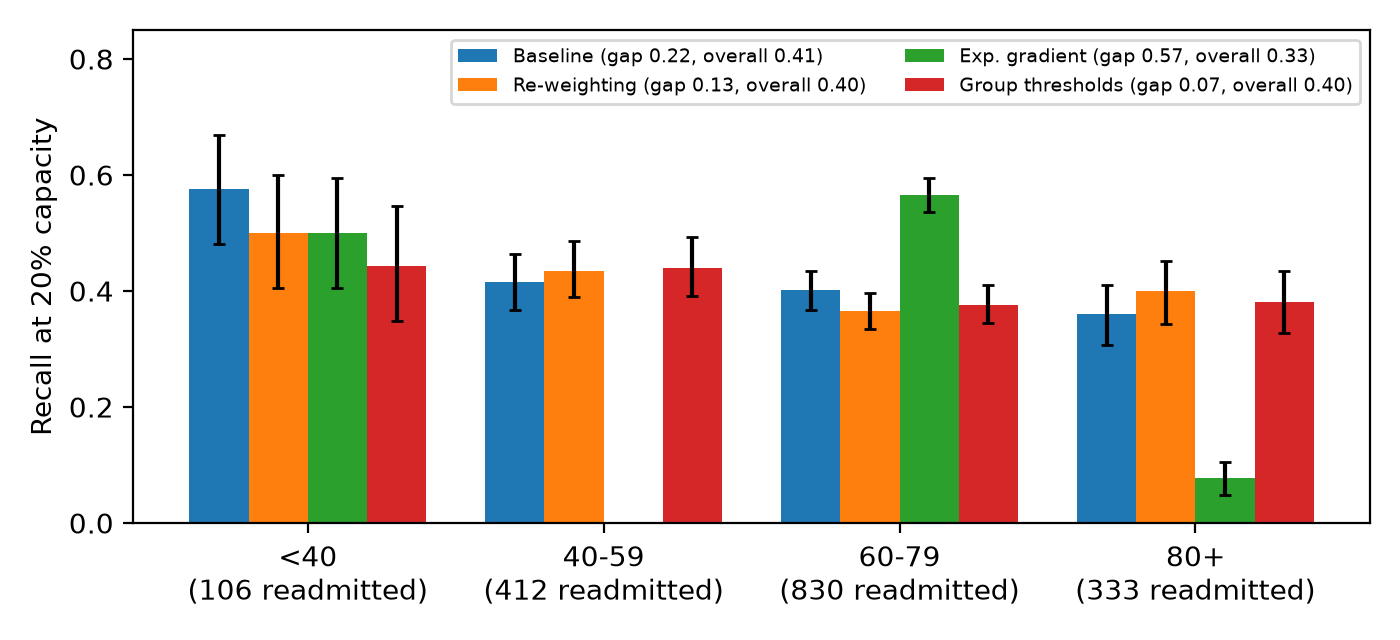
\includegraphics[width=0.78\textwidth]{fairness_recall_by_age.png}
\caption{Recall at 20\% capacity by age group for each mitigation (95\% bootstrap confidence intervals).}\label{fig:3}
\end{figure}


\lead{What we learned:}
\begin{itemize}
\item \textbf{Per-age-group thresholds work best.} Thresholds fitted on the validation set give each age band the same recall while keeping the total number flagged at capacity. Recall for 80+ rises from 36\% to 38\%, the gap is no longer significant, and overall recall falls by only 1.1 points (about 18 of 1,681 readmissions). This method treats age groups explicitly differently. We consider this acceptable because age is a clinically legitimate factor and the adjustment \emph{raises} priority for the group that was being missed. It still requires approval by the governance committee.
\item \textbf{Fixing one attribute can strain another.} Re-weighting narrowed the age gap but not enough (still significant), and it widened the sex gap from 1.8 to 4.4 points (p = 0.06, borderline). In an earlier version of our prototype the same method made the sex gap significant. Checking every attribute after every change is essential.
\item \textbf{Constraint methods must match how the model is used.} Exponentiated gradient enforces equal recall at the classifier's own decision threshold. SafeDischarge instead flags a fixed top 20\%. At that operating point the constrained model was both less accurate and \emph{less} fair. Fairness must be evaluated at the operating point actually deployed.
\item \textbf{Leaving race out of the model is not enough} on its own~\cite{chen2018}. That is why race is still audited.
\end{itemize}

\subsection{Privacy preservation}\label{sec:4.3}

\textbf{Why it matters:} hospital records are highly sensitive. Pooling them needs legal agreements and increases the damage from a breach. Trained models can also reveal whether a person was in the training data (membership inference)~\cite{shokri2017}.

\lead{Mechanisms:}
\begin{enumerate}
\item \textbf{Federated learning:} patient records never leave a hospital; only model updates do.
\item \textbf{Secure aggregation:} the server sees only masked updates and learns only their sum (Section~\ref{sec:3.4}).
\item \textbf{Differential privacy:} each hospital trains with \textbf{DP-SGD}~\cite{abadi2016} in Opacus~\cite{yousefpour2021}. Each patient's gradient is clipped (norm 1.0) and Gaussian noise is added. The noise level is set by Opacus's privacy accountant so that each hospital spends at most the target ε over all 20 rounds (δ = 10\textsuperscript{−5}).
\item \textbf{Data minimisation and local scoring:} only fields needed for prediction are used, the data is de-identified, and daily scoring runs inside each hospital.
\item \textbf{Privacy attack test:} a loss-threshold membership-inference attack~\cite{yeom2018} tries to tell training patients from unseen patients. An AUC of 0.5 means it can do no better than guessing.
\end{enumerate}

\textbf{Results (Table~\ref{tab:4}, Figure~\ref{fig:4}).}
\begin{itemize}
\item \textbf{The attack works when a model leaks:} against a deliberately over-fitted model it reaches AUC 0.592.
\item \textbf{Normal models leak a little:} pooled and federated models without DP give AUC 0.508–0.511.
\item \textbf{DP removes measurable leakage:} at every ε tested the attack is at chance (0.499–0.500).
\item \textbf{Accuracy cost:} 1.2 AUROC points at ε = 8 and 1.7 at ε = 3. At ε = 8 the shared model is slightly better than the average hospital training alone (0.662 vs 0.660), though not better than the largest hospital alone (0.666). At ε = 3 it is slightly below the average single hospital, but with a much stronger privacy guarantee. Most of the federation gain is spent on privacy.
\item \textbf{Recommended setting:} ε = 8. It is the strongest guarantee we tested that keeps a small benefit over training alone for most hospitals. ε = 3 is the conservative alternative.
\end{itemize}
\begin{figure}[htbp]
\centering
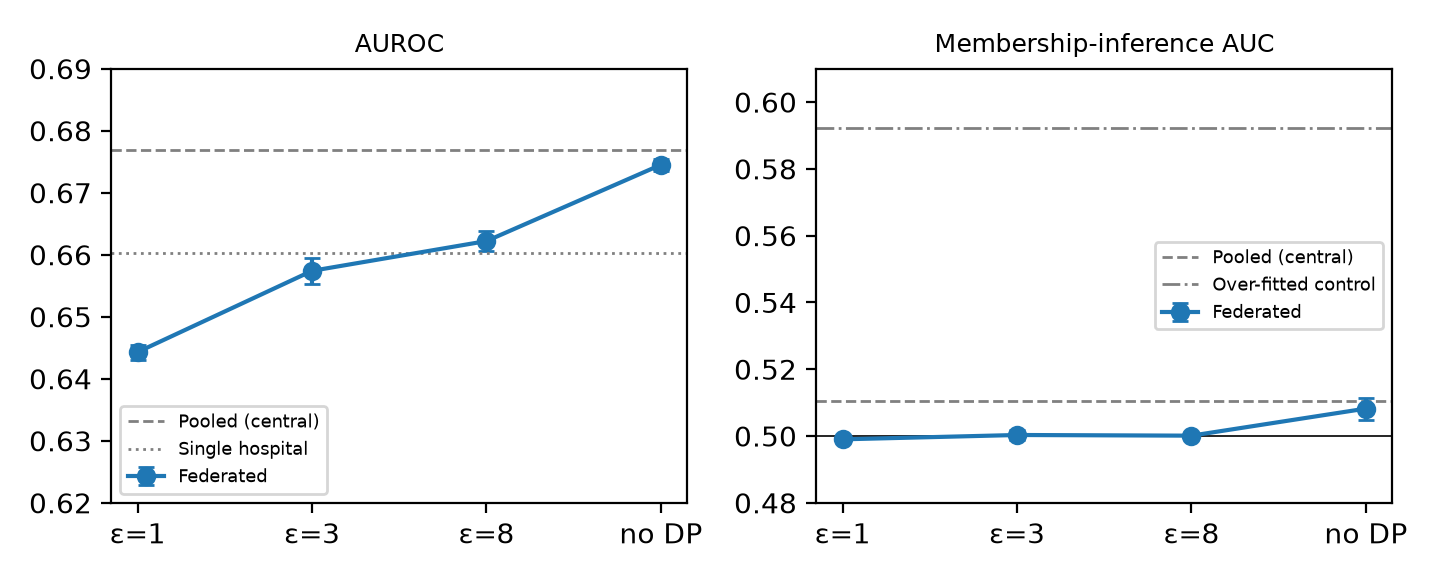
\includegraphics[width=0.78\textwidth]{privacy_tradeoff.png}
\caption{Privacy–utility trade-off: AUROC (left) and membership-inference AUC (right) for federated training at ε = 1, 3, 8 and without DP (mean ± SD, 3 seeds).}\label{fig:4}
\end{figure}


\subsection{Trade-offs and the release gate}\label{sec:4.4}
\begin{itemize}
\item \textbf{Privacy vs fairness.} DP is known to hurt small groups most~\cite{bagdasaryan2019}. In our runs the opposite happened for age: the DP models had a \emph{smaller} age gap (6–10 points vs 23 without DP), probably because the noise stops the model relying heavily on age-specific patterns. This is one dataset and one model, so the release gate re-tests fairness after DP rather than assuming either direction.
\item \textbf{Fairness vs accuracy.} Equalising recall across age groups costs 1.1 points of overall recall.
\item \textbf{Accuracy vs explainability.} The more complex model is accepted only because it beats the interpretable baseline by more than the agreed margin.
\end{itemize}

\textbf{Release gate.} A new model version is deployed only if:
\begin{enumerate}
\item recall at capacity is no worse than the current model;
\item no protected attribute shows a significant recall gap (permutation p ≥ 0.05), and small groups are listed as “insufficient data”;
\item ε is within the agreed budget and the membership-inference AUC is ≤ 0.52;
\item the governance committee signs off the global explanations and any group-specific thresholds;
\item the model card is updated.
\end{enumerate}

\subsection{Accountability and human oversight}\label{sec:4.5}
\begin{itemize}
\item \textbf{The nurse decides.} SafeDischarge only prioritises extra follow-up. No patient loses standard discharge care, and a nurse can add any patient to the list.
\item \textbf{Overrides are logged and reviewed.} Every accept or override is recorded with a reason. Override rates are reviewed monthly by patient group; a group whose flags are often overridden triggers a review of the model or the action table.
\item \textbf{Patients can ask why.} Patients are told that a decision-support tool is used, and can ask why they were or were not offered follow-up. Staff answer using the same plain-language reasons the nurse sees.
\item \textbf{Clear ownership.} The governance committee owns each release. Every model version is stored with its data snapshot, ε spent, fairness results and model card, so any past decision can be traced to the model that made it.
\end{itemize}
\begin{table}[htbp]
\centering
\caption{Summary: Responsible AI mechanisms and measured results.}\label{tab:6}
\begin{tabularx}{\textwidth}{>{\raggedright\arraybackslash\hsize=0.459\hsize}X>{\raggedright\arraybackslash\hsize=1.384\hsize}X>{\raggedright\arraybackslash\hsize=1.158\hsize}X}
\toprule
\textbf{Practice} & \textbf{Mechanisms} & \textbf{Measured result} \\
\midrule
Explainability & SHAP top-3 reasons → actions, faithfulness test, calibration, interpretable baseline, global review, model card & Removing top-3 reasons cuts risk 29\% vs 2.7\% for random variables; Brier 0.215 → 0.095 \\
Fairness & Equal-opportunity audit, permutation test, per-age-group thresholds, re-testing every attribute & Age gap 21.5 → 6.8 pts (p < 0.001 → 0.39) for −1.1 pts recall \\
Privacy & Federated learning, secure aggregation, DP-SGD with accountant, local scoring, attack test & Federated ≈ pooled (0.675 vs 0.677); DP ε = 8 costs 1.2 pts; attack AUC 0.508 → 0.500 \\
\bottomrule
\end{tabularx}
\end{table}


\section{Limitations}\label{sec:5}
\begin{itemize}
\item \textbf{Old, US-only data.} The dataset covers 1999–2008 in the US. Practice and populations have changed. A real deployment must retrain and validate on current local data.
\item \textbf{Simulated hospitals.} Without hospital IDs, the virtual-hospital split approximates real between-site differences but cannot reproduce them fully.
\item \textbf{Simulated secure aggregation.} The masking protocol is simulated in one process. Real deployments need the full cryptographic protocol, including handling hospitals that drop out mid-round.
\item \textbf{Modest accuracy.} AUROC ≈ 0.68. SafeDischarge is a prioritisation aid, not an automated decision-maker.
\item \textbf{Prediction is not prevention.} Benefit depends on the follow-up actions working. A prospective before/after evaluation is needed.
\item \textbf{Small groups.} Several race groups have too few readmissions to audit. Collaborating hospitals with more diverse populations are needed to check fairness for them.
\end{itemize}

\section{Conclusion}\label{sec:6}

SafeDischarge helps discharge teams direct limited follow-up resources to the diabetic patients most likely to be readmitted. The prototype shows the design is practical: on public data, it doubles the readmissions caught compared with random selection. Its explanations pass a faithfulness test, and its audit found and fixed an age disparity that would have left the oldest patients under-served. Federated training gives every hospital close to pooled-data accuracy without pooling records, and differential privacy removes measurable leakage at a cost of about one AUROC point. Each Responsible AI practice is a tested mechanism enforced by a release gate.

\vspace{4pt}
\noindent\textbf{Use of AI tools.} An AI assistant (Claude, Anthropic) was used to help write and debug the prototype code and to edit the report text. The author designed the system, chose the methods, checked every result against the prototype's output files, and takes responsibility for the content.

% ---------------- References ----------------
\begin{thebibliography}{99}
\setlength{\itemsep}{1pt}
\bibitem{cms-hrrp} Centers for Medicare \& Medicaid Services. \emph{Hospital Readmissions Reduction Program (HRRP)}. \url{https://www.cms.gov/medicare/payment/prospective-payment-systems/acute-inpatient-pps/hospital-readmissions-reduction-program-hrrp}
\bibitem{vanwalraven2010} C. van Walraven et al. Derivation and validation of an index to predict early death or unplanned readmission after discharge from hospital to the community. \emph{CMAJ}, 182(6), 2010.
\bibitem{donze2013} J. Donzé, D. Aujesky, D. Williams, J. L. Schnipper. Potentially avoidable 30-day hospital readmissions in medical patients: derivation and validation of a prediction model. \emph{JAMA Internal Medicine}, 173(8), 2013.
\bibitem{kansagara2011} D. Kansagara et al. Risk prediction models for hospital readmission: a systematic review. \emph{JAMA}, 306(15), 2011.
\bibitem{obermeyer2019} Z. Obermeyer, B. Powers, C. Vogeli, S. Mullainathan. Dissecting racial bias in an algorithm used to manage the health of populations. \emph{Science}, 366(6464), 2019.
\bibitem{rajkomar2018} A. Rajkomar, M. Hardt, M. D. Howell, G. Corrado, M. H. Chin. Ensuring fairness in machine learning to advance health equity. \emph{Annals of Internal Medicine}, 169(12), 2018.
\bibitem{strack2014} B. Strack, J. P. DeShazo, C. Gennings, J. L. Olmo, S. Ventura, K. J. Cios, J. N. Clore. Impact of HbA1c measurement on hospital readmission rates: analysis of 70,000 clinical database patient records. \emph{BioMed Research International}, 2014. Dataset: UCI Machine Learning Repository, “Diabetes 130-US Hospitals for Years 1999–2008”, CC BY 4.0.
\bibitem{pedregosa2011} F. Pedregosa et al. Scikit-learn: Machine learning in Python. \emph{Journal of Machine Learning Research}, 12, 2011.
\bibitem{lundberg2017} S. M. Lundberg, S.-I. Lee. A unified approach to interpreting model predictions. \emph{NeurIPS}, 2017.
\bibitem{bird2020} S. Bird et al. Fairlearn: A toolkit for assessing and improving fairness in AI. Microsoft Technical Report MSR-TR-2020-32, 2020.
\bibitem{yousefpour2021} A. Yousefpour et al. Opacus: User-friendly differential privacy library in PyTorch. arXiv:2109.12298, 2021.
\bibitem{mcmahan2017} B. McMahan, E. Moore, D. Ramage, S. Hampson, B. A. y Arcas. Communication-efficient learning of deep networks from decentralized data. \emph{AISTATS}, 2017.
\bibitem{beutel2020} D. J. Beutel et al. Flower: A friendly federated learning research framework. arXiv:2007.14390, 2020.
\bibitem{bonawitz2017} K. Bonawitz et al. Practical secure aggregation for privacy-preserving machine learning. \emph{ACM CCS}, 2017.
\bibitem{hardt2016} M. Hardt, E. Price, N. Srebro. Equality of opportunity in supervised learning. \emph{NeurIPS}, 2016.
\bibitem{chen2018} I. Chen, F. D. Johansson, D. Sontag. Why is my classifier discriminatory? \emph{NeurIPS}, 2018.
\bibitem{shokri2017} R. Shokri, M. Stronati, C. Song, V. Shmatikov. Membership inference attacks against machine learning models. \emph{IEEE S\&P}, 2017.
\bibitem{abadi2016} M. Abadi et al. Deep learning with differential privacy. \emph{ACM CCS}, 2016.
\bibitem{yeom2018} S. Yeom, I. Giacomelli, M. Fredrikson, S. Jha. Privacy risk in machine learning: analyzing the connection to overfitting. \emph{IEEE CSF}, 2018.
\bibitem{bagdasaryan2019} E. Bagdasaryan, O. Poursaeed, V. Shmatikov. Differential privacy has disparate impact on model accuracy. \emph{NeurIPS}, 2019.
\end{thebibliography}

\end{document}
